\section{Architecture}
\label{sec:architecture}

Being a blockchain project, the goal is to not use the so called Web2
technologies, this means the traditional approaches of having a backend running
on a server and similar services, but rather to use only Web3 technologies for
us to understand exactly the limitations there are by adopting solely the
blockchain ecosystem. Ideally, of course, in the future this project benefits
greatly by merging these two approaches.

The system's architecture is illustrated in Figure \ref{fig:architecture},
showing how each component of the project interacts, aligned with the
requirements discussed in previous sections.

\begin{figure}[H]
    \centering
    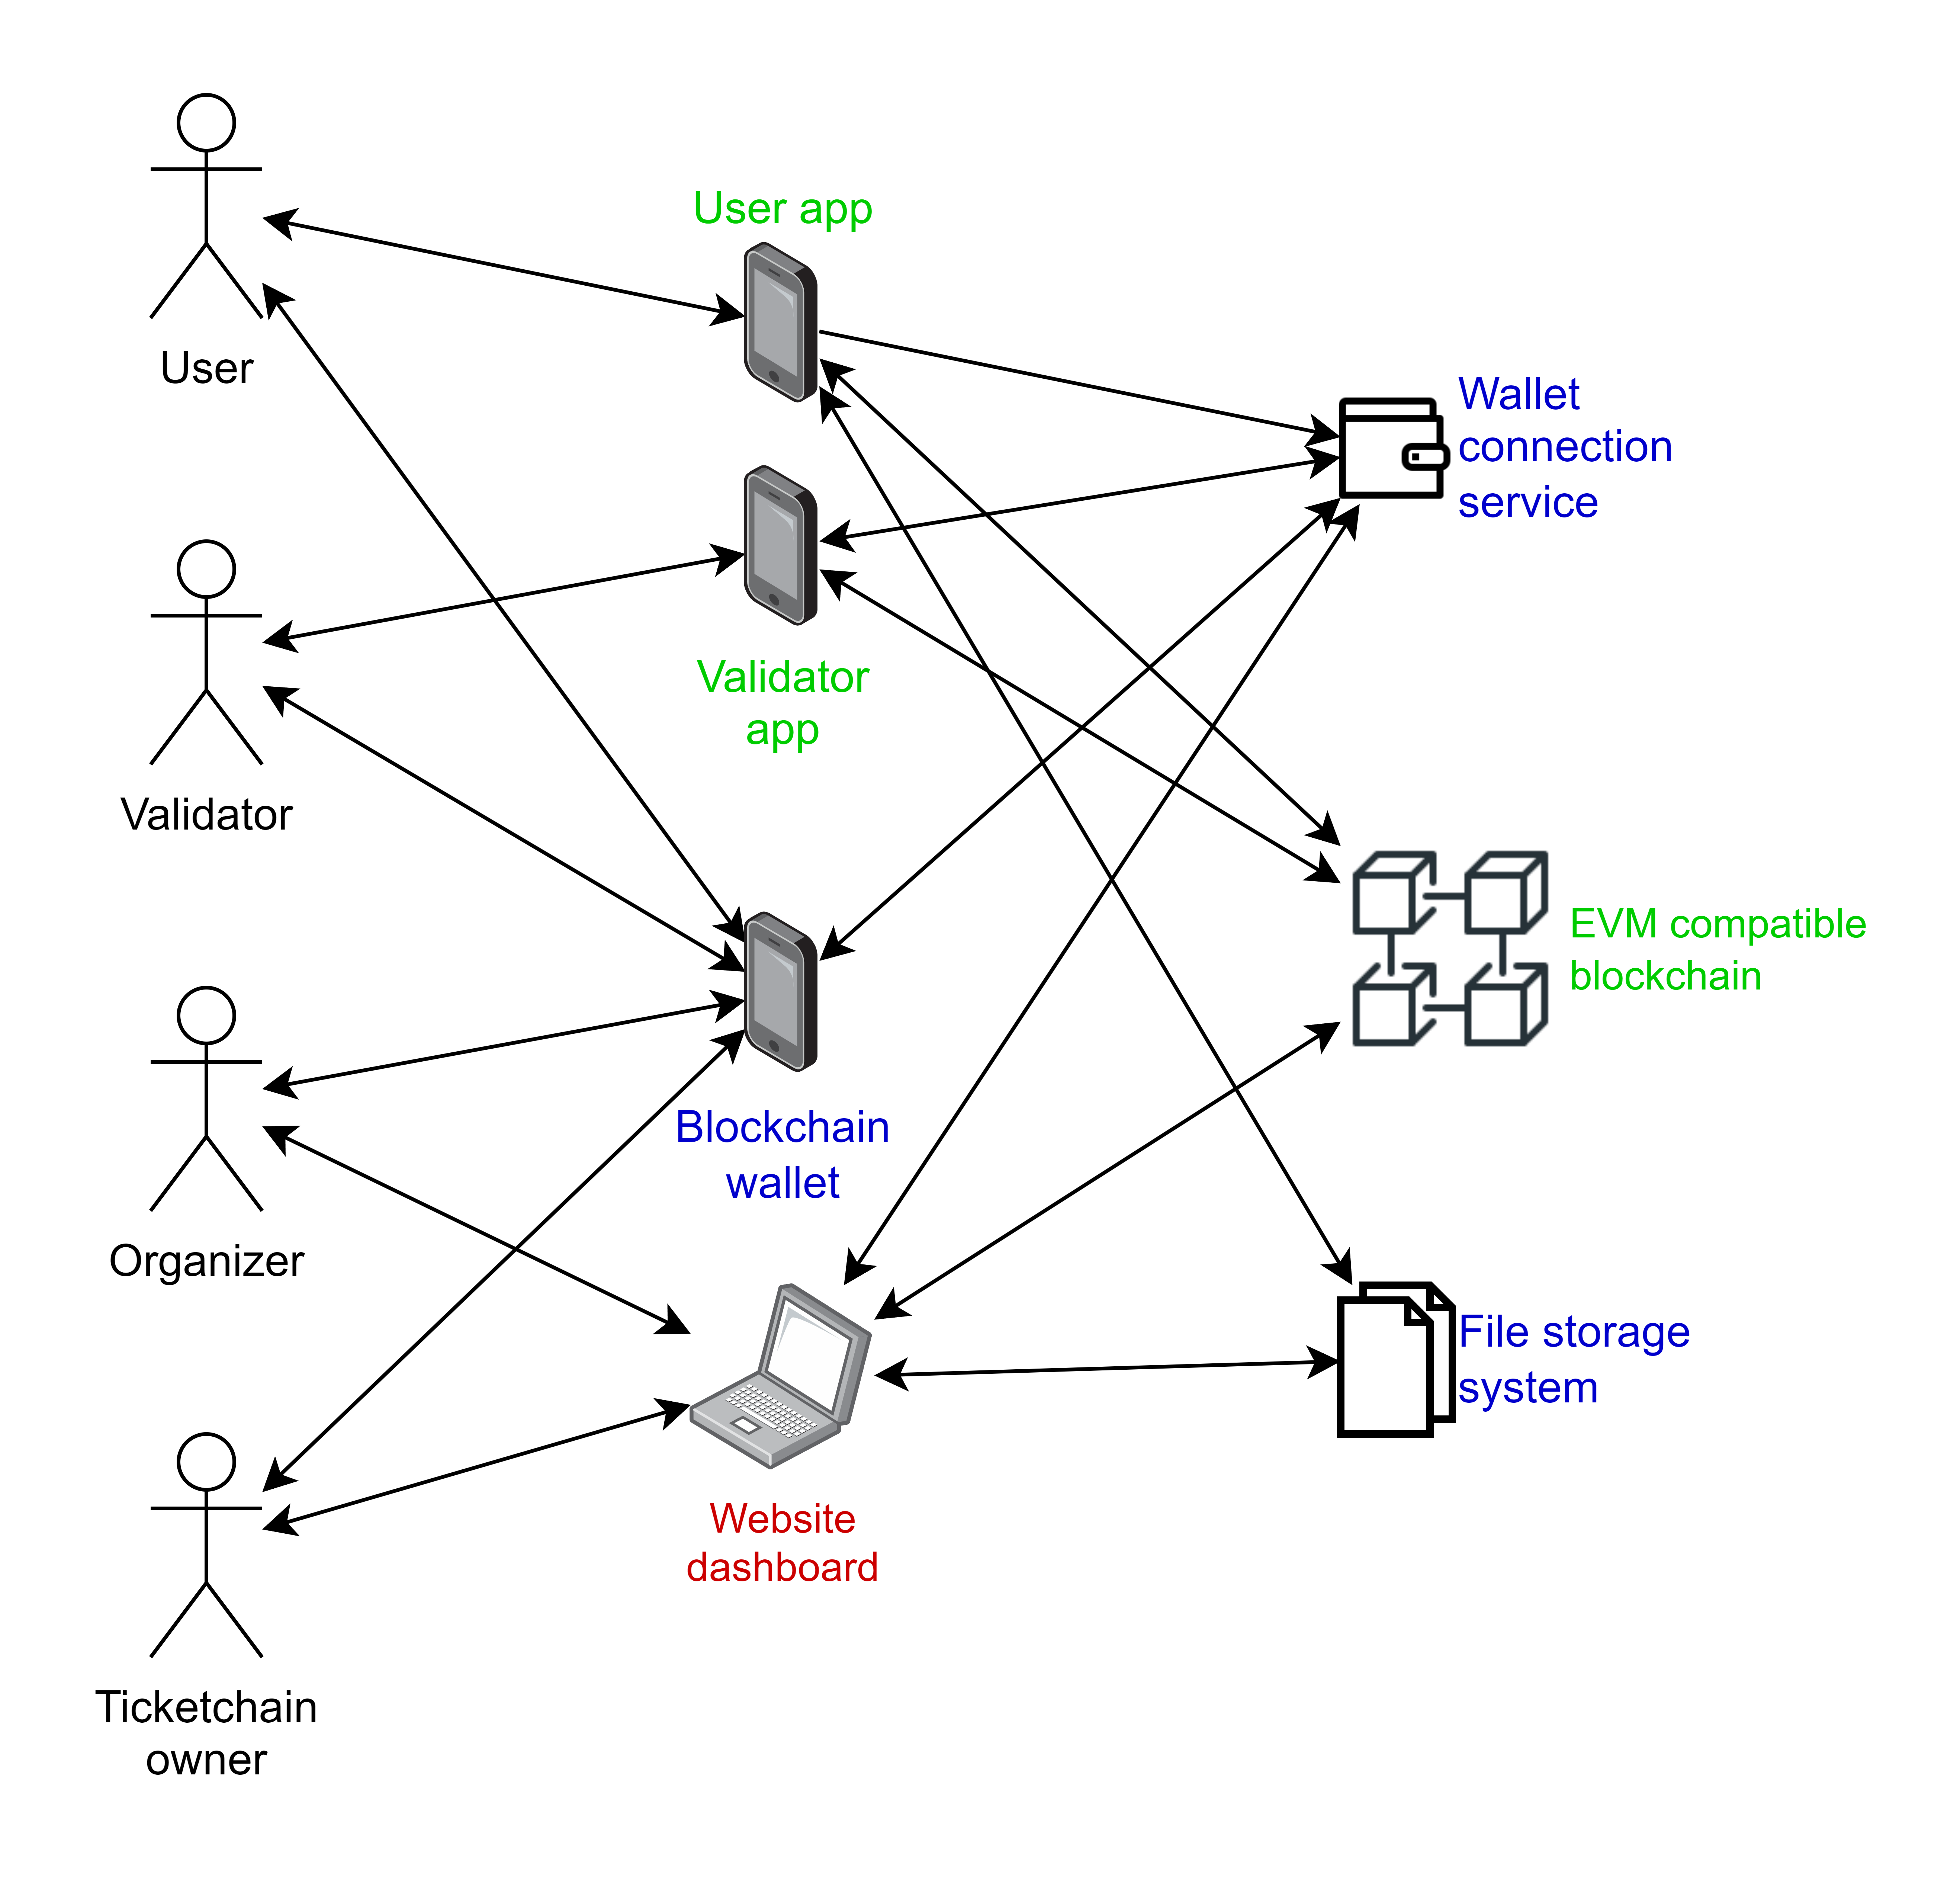
\includegraphics[width=0.66\textwidth]{Architecture.png}
    \caption{System Architecture}
    \label{fig:architecture}
\end{figure}

The architecture comprises a mobile application for both common users and
validators, as well as a web dashboard for the Ticketchain owner and event
organizers to manage system settings and events. Due to time constraints, this
part of the system has not yet been implemented; for now, interactions will be
conducted directly with the smart contract.

As detailed in the use cases section, all users must authenticate before
accessing the system. Instead of a traditional login using email and password,
authentication will require wallet software to interact with the blockchain.
Therefore, a wallet connection service is necessary to link users' wallets to
the system.

Once the wallet connection is established, the system will communicate with the
smart contract to display event-related information and update the status of
events or tickets. The entire codebase will be deployed on an EVM-compatible
blockchain. For ticket images, a file storage system will be needed. While
image uploads will typically be managed through the dashboard, this feature has
yet to be implemented, necessitating manual uploads for the time being.
